\documentclass[lettersize,journal]{IEEEtran}

\usepackage{amsmath,amsfonts,amssymb}
\usepackage{array}
\usepackage{stfloats}
\usepackage{url}
\usepackage{graphicx}
\usepackage{cite}
\hyphenation{op-tical net-works semi-conduc-tor IEEE-Xplore}
\def\BibTeX{{\rm B\kern-.05em{\sc i\kern-.025em b}\kern-.08em
    T\kern-.1667em\lower.7ex\hbox{E}\kern-.125emX}}

\urlstyle{same}

% Float spacing: IEEEtran defaults leave generous gaps around floats.
% Tightened to recover vertical space without altering figure content.
\setlength{\textfloatsep}{4pt plus 1pt minus 1pt}
\setlength{\floatsep}{6pt plus 2pt minus 2pt}
\setlength{\intextsep}{6pt plus 2pt minus 2pt}
\setlength{\dbltextfloatsep}{4pt plus 1pt minus 1pt}
\setlength{\dblfloatsep}{6pt plus 2pt minus 2pt}
\setlength{\abovecaptionskip}{3pt}
% Float packing: IEEEtran's defaults reserve a large fraction of each
% column for text, which strands whitespace on figure-heavy pages.
% Raising the float fractions lets LaTeX fill those pages properly.
\renewcommand{\topfraction}{0.95}
\renewcommand{\bottomfraction}{0.95}
\renewcommand{\textfraction}{0.05}
\renewcommand{\floatpagefraction}{0.85}
\renewcommand{\dbltopfraction}{0.95}
\renewcommand{\dblfloatpagefraction}{0.85}
\setlength{\belowcaptionskip}{0pt}

\begin{document}

\title{Second-Order Cooperative Field Estimation for
Multirobot Tracking of Coherent Flow Structures}

\author{Christopher Waight and Christopher A. Kitts,~\IEEEmembership{Senior Member,~IEEE}
\thanks{C. Waight is a PhD Candidate in the Robotic Systems Laboratory, Department of Mechanical Engineering, Santa Clara University, Santa Clara, CA 95053 USA (e-mail: cwaight@scu.edu)}
\thanks{C. A. Kitts is Professor and Director of the Robotic Systems Laboratory, Department of Mechanical Engineering, Santa Clara University, Santa Clara, CA 95053 USA (e-mail: ckitts@scu.edu)}
}
\markboth{IEEE Systems Journal}%
{Waight and Kitts: Second-Order Cooperative Field Estimation for Multirobot Tracking of Coherent Flow Structures}

\maketitle

\begin{abstract}
Adaptive navigation is the process of modifying a robot's or a system of robots' motion in
real time based on measurements taken while moving. This paper applies
that process to the boundaries that organize short-term transport in a
flow, such as the strain-dominated curves across which water masses separate
and along which floating material collects. Existing robotic trackers
of such structures either commit to the structure's identity and pre-straddle it before
tracking begins or accumulate an estimate over a finite integration
horizon. We show that a second-order fit of the local flow can remove both
requirements. A cooperative estimator recovers the local quadratic field
model from one synchronized set of measurements, six robots being the minimum
for the unconstrained model. This quadratic model can be used as the foundation to create surrogate
fields. We build an adaptive navigation primitive to steer on each of two
such surrogate fields, the Jacobian determinant and the smaller
rate-of-strain eigenvalue. Each locates a separating boundary and navigates to and along
it from instantaneous measurements, with no integration horizon and no
pre-straddling. The choice of surrogate sets a tradeoff. Monte Carlo
sweeps from seven starts, four of them off the structure, show that the determinant tracker withstands
more measurement noise than the strain tracker from every start. In a rotating-frame trial only the strain
tracker, which is objective, holds the same material path. On Santa
Barbara Channel radar currents, both primitives follow the same dominant
transport corridor.

\end{abstract}

\begin{IEEEkeywords}
Mobile Robots, Multirobot Systems, Adaptive Navigation, Coherent
Structures, Rate of Strain, Objectivity, Cooperative Estimation,
Cluster Space Control
\end{IEEEkeywords}

\section{Introduction}

\IEEEPARstart{M}{ultirobot} systems (MRS) offer redundancy, increased
throughput, and cooperative behaviors a single vehicle cannot produce,
and they now operate across land, sea, air, and space \cite{1,2}.
 In adaptive
navigation (AN), a vehicle or group of vehicles modifies its direction and path in real time
from measurements taken while moving \cite{3}. A single vehicle must translate to sense a
gradient, which costs time and misleads in a time-varying field,
whereas an MRS can sample multiple locations simultaneously, tolerate
vehicle failures, adapt its size and shape to the spatial frequencies
present, and fit a local model of the landscape to steer on its features
\cite{3,4,5}.

AN in scalar fields is well developed. Each
robot contributes one scalar measurement to a policy that reaches and
follows a feature, and formations are sized so that differential
measurements across the cluster recover the gradient and curvature that
policy consumes \cite{5,6}. \"{O}gren, Fiorelli, and Leonard
established cooperative gradient climbing with a formation of mobile
sensors \cite{6}. Bri\~{n}\'{o}n-Arranz, Renzaglia, and Schenato
extended it to the Hessian, five robots on a ring plus one at the
center recovering both in closed form \cite{5}. Kitts, McDonald, and
Neumann developed primitives for extrema finding, contour following,
ridge/trench following, and saddle point station keeping \cite{3}, and
verified ridge, trench, saddle, and front tracking experimentally on an
indoor testbed \cite{4,7}.

Some environments are better modeled as vector fields, which contain features without scalar field equivalents. Critical points, such as sinks, sources, and vortices, can model convergence zones \cite{8} and subsurface leaks \cite{9}.  In \cite{10} a three-robot cluster
estimated the location and type of one from a linear fit of
simultaneous local velocity measurements and used this estimate to adaptively navigate towards and around them. 

Beyond critical points, vector fields have curves that are useful for navigation. For example, dynamic ocean flows contain naturally occurring boundaries known as coherent structures that influence where floating materials like debris and larvae will accumulate or separate \cite{11,12}. Mapping these exact curves allows teams to strategically deploy resources in highly targeted search areas \cite{12,13,14,15}. Without adaptive navigation, a large scale team must sample a much larger basin to determine where these structures lie.

Coherent structures are typically identified through two primary methods. The first relies on Lagrangian coherent structures (LCS) \cite{16}, typically computed as ridges in the finite-time Lyapunov exponent field \cite{17}, with ongoing research addressing the Lagrangian/Eulerian tradeoff and sparse-trajectory gradient recovery \cite{18,19,20,21}. The second method uses instantaneous Eulerian criteria, such as the Okubo-Weiss parameter, to partition flows based solely on the local velocity gradient \cite{8,22}. This instantaneous approach has been generalized to three dimensions \cite{23}, refined to second order \cite{24}, and applied at scale in mesoscale eddy censuses \cite{25}. However, both of these methods characterize these structures offline using a reconstructed field, which is not well suited to real-time adaptive navigation of a field that evolves in time.  

New work is being done on using AN techniques with MRS in these scenarios. Michini et al. bracket a presumed stable or
unstable manifold with three robots using only local velocity
measurements \cite{26}, an approach inspired by the PIM triple
procedure, extended to $N$ robots \cite{27} and validated
experimentally in gyre-like flows \cite{28}. The robots begin on the
manifold and are advected by the flow, and the manifold's identity is
supplied in advance. The saddle point is treated by neither the
controller nor its analysis, and that work reports veering away from
the structure near a saddle in flow-tank experiments. Kularatne and Hsieh confirm the boundary by computing the local FTLE field on board, at the cost of a nonzero integration horizon and a commitment to attracting structures \cite{29}. In both cases, the robotic formation pre-straddles the structure, and does not acquire a structure it does not already occupy.

This paper shows that a second-order fit of the local flow can be used to
acquire and track such a structure from instantaneous measurements. A
linear fit, as in \cite{10}, gives the velocity gradient at one point. A
second-order fit gives it as a field over the formation, so any quantity
built from it comes with its own gradient in closed form. The contributions are
\begin{itemize}
\item a cooperative estimator that recovers the local quadratic model of
a two-component field from one synchronized set of measurements across six robots, the
minimum for the unconstrained model, and that fails only when the robots
lie on a common conic;
\item two surrogates read in closed form from that fit, the
velocity-gradient determinant $D$ and the smaller strain eigenvalue
$s_1$ \cite{19};
\item two AN primitives, the $D$ tracker and the $s_1$ tracker, that
navigate to the structure and ride along it without pre-straddling;
\item a tradeoff between them, in which the $D$ tracker tolerates more
measurement noise while the $s_1$ tracker, being objective, holds its
path under a rotating observer, which matters when the measured flow
carries the observer's own rotation.
\end{itemize}

Both primitives run on a simulated double gyre and on measured Santa
Barbara Channel radar currents.

\section{Second-Order Field Estimation}

\subsection{Local Vector Field Polynomials}

A planar vector field assigns a velocity $\mathbf{v}(\mathbf{p}) =
(u(\mathbf{p}), v(\mathbf{p}))$ to each position in space $\mathbf{p} = (x, y)$.
The critical point estimator of \cite{10} fits a plane to each
component of the vector field and solves for the point where $\mathbf{v} = \mathbf{0}$. 

In this work, we extend the linear approximation to the second-order Taylor expansion about the
centroid, $\mathbf{p}_c$. Coordinates are measured
from the centroid throughout this section, so $\mathbf{p}_c = \mathbf{0}$.
\begin{align}
    u(\mathbf{p}) &= a_1 + a_2 x + a_3 y
        \nonumber \\
        &\quad + a_4 xy + \tfrac{1}{2} a_5 x^2 + \tfrac{1}{2} a_6 y^2
        + \mathcal{O}(\|\mathbf{p}\|^3),
        \label{eq:quad_model_u} \\
    v(\mathbf{p}) &= b_1 + b_2 x + b_3 y
        \nonumber \\
        &\quad + b_4 xy + \tfrac{1}{2} b_5 x^2 + \tfrac{1}{2} b_6 y^2
        + \mathcal{O}(\|\mathbf{p}\|^3),
        \label{eq:quad_model_v}
\end{align}
where $\mathcal{O}(\|\mathbf{p}\|^3)$ is the truncation error.
The twelve coefficients of this quadratic model are constants and each is a derivative of the field at
the centroid. The one-half factors cancel the factor of 2 during differentiation.
This gives $a_1 = u(\mathbf{p}_c)$, $a_2 = \partial u/\partial
x|_{\mathbf{p}_c}$, $a_3 = \partial u/\partial y|_{\mathbf{p}_c}$,
$a_4 = \partial^2 u/\partial x \partial
y|_{\mathbf{p}_c}$, $a_5 = \partial^2 u/\partial x^2|_{\mathbf{p}_c}$,
$a_6 = \partial^2 u/\partial y^2|_{\mathbf{p}_c}$,
and likewise for $b_1, \ldots, b_6$ with $v$ in place of $u$.

To estimate these coefficients with robot positions $\mathbf{p}_i = (x_i,
y_i)$, we define the quadratic basis vector
\begin{equation}
    \boldsymbol{\phi}(\mathbf{p}) =
    \bigl[\,1, \; x, \; y, \; xy, \;
    \tfrac{1}{2}x^2, \; \tfrac{1}{2}y^2\,\bigr]^\top,
\end{equation}
whose entries are the terms of
(\ref{eq:quad_model_u})--(\ref{eq:quad_model_v}) in order, so
the recovered coefficients, which we mark with a hat, estimate the Taylor derivatives directly with
no rescaling. Stacking the six basis vectors row-wise gives
the $6 \times 6$ formation matrix $\boldsymbol{\Phi}$, and the coefficient
estimates $\hat{\boldsymbol{\theta}}_u = [\hat{a}_1, \ldots,
\hat{a}_6]^\top$ and $\hat{\boldsymbol{\theta}}_v = [\hat{b}_1, \ldots,
\hat{b}_6]^\top$ solve
\begin{equation}
    \boldsymbol{\Phi}\,\hat{\boldsymbol{\theta}}_u = \mathbf{m}_u, \qquad
    \boldsymbol{\Phi}\,\hat{\boldsymbol{\theta}}_v = \mathbf{m}_v,
    \label{eq:solve}
\end{equation}
where $\mathbf{m}_u = [u_1, \ldots, u_6]^\top$ and
$\mathbf{m}_v = [v_1, \ldots, v_6]^\top$ collect the measurements $u_i$ and $v_i$, the components of the velocity
sampled by robot $i$. 

\subsection{Minimality}
\label{sec:minimality}

Six robots is the minimum for recovery of the unconstrained local
quadratic model of a two-component planar field from one synchronized set of measurements. Each robot contributes one equation per component to
(\ref{eq:solve}), and each system has six unknowns, so fewer than six
robots leave the solution set a positive-dimensional affine subspace.

Six robots suffice provided $\boldsymbol{\Phi}$ is nonsingular. With
more than six, $\boldsymbol{\Phi}$ has more rows than columns, the fit
becomes least squares, and the condition becomes full column rank.
Either condition fails exactly when the robots lie on a common conic.
For example, a standard ring formation is degenerate at any size, since
the ring itself is the conic. A fit from more than six robots also
leaves a residual, which carries the measurement noise and the
truncation error.

With five equations or fewer, a method either returns a family of solutions or imposes a structural prior, such as assuming
divergence-free flow by imposing $\nabla\cdot\mathbf{v} = 0$. We do not impose any priors on the field, as horizontal surface
currents are not divergence free, so imposing
$\nabla\cdot\mathbf{v} = 0$ would bias every recovered coefficient.

For this study, we chose the pentagon-plus-center formation and use it
throughout. It is the smallest uniform ring plus center on which \cite{5}
recovers a scalar Hessian exactly for quadratic signals, independent of
the formation's orientation. The same symmetry makes the noise gains of
the fit here independent of formation heading.


\subsection{Estimator Sensitivity}
\label{sec:sensitivity}

The accuracy of the estimator is affected by the formation of the
robots, the noise on each robot's measurements, and the error in each
robot's position.

\subsubsection{Formation}
The rank of the formation matrix $\boldsymbol{\Phi}$ determines whether
a unique fit exists, and its condition number $\kappa(\boldsymbol{\Phi})$
indicates how much the fit amplifies noise. Condition numbers are
reported on the radius-normalized $\boldsymbol{\Phi}$, with each column
of order $q$ divided by $\rho^{\,q}$, where $\rho$ is the formation radius. Without this normalization, the
quadratic columns shrink as $\rho^{2}$ and a healthy formation would
appear degenerate. The normalized matrix depends only on the formation's
shape, and the pentagon-plus-center formation gives
$\kappa(\boldsymbol{\Phi}) = 8.26$ at every radius. The size of the formation instead scales the noise on each
coefficient by $\rho^{-q}$, so a larger formation suppresses noise most
in the second-order terms. The condition number grows as the robots
drift toward a common conic. For example, moving the center robot out
to $0.99\rho$ places all six robots within $0.6\%$ of a common circle
and raises $\kappa(\boldsymbol{\Phi})$ to $564$. The fit degrades
continuously on the way to the degeneracy of
Section~\ref{sec:minimality}, with no threshold at which it fails.

\subsubsection{Measurement Noise}
Each robot carries its own sensor, so the measurement noise of one robot
is independent of the others. Furthermore, the estimator uses only
instantaneous readings, so each cycle's fit sees only that cycle's
noise. The noise is modeled as additive on each reading,
\begin{equation}
    u_i^m = u(\mathbf{p}_i) + \eta_i^u, \qquad
    v_i^m = v(\mathbf{p}_i) + \eta_i^v,
    \label{eq:meas_noise}
\end{equation}
with $\eta \sim \mathcal{N}(0, \sigma_{uv}^2)$. The fit is linear in the
measurements, so the noise reaches the coefficients as
$\boldsymbol{\Phi}^{-1}\boldsymbol{\eta}^u$ and
$\boldsymbol{\Phi}^{-1}\boldsymbol{\eta}^v$, where $\boldsymbol{\eta}^u$
and $\boldsymbol{\eta}^v$ stack the noise of the six robots. Both are
zero-mean, so measurement noise adds no bias to the coefficient estimates.

\subsubsection{Position Noise}
A robot with position error
$\boldsymbol{\xi}_i \sim \mathcal{N}(\mathbf{0}, \sigma_p^2\mathbf{I})$
samples the field at $\mathbf{p}_i + \boldsymbol{\xi}_i$, but the fit is
built from its nominal position $\mathbf{p}_i$. The formation matrix is
therefore wrong by $\Delta\boldsymbol{\Phi}$, whose row $i$ is
$\boldsymbol{\phi}(\mathbf{p}_i + \boldsymbol{\xi}_i)^{\top} -
\boldsymbol{\phi}(\mathbf{p}_i)^{\top}$. Under the quadratic model the
measurements are
$\mathbf{m}_u = (\boldsymbol{\Phi} + \Delta\boldsymbol{\Phi})
\boldsymbol{\theta}_u$, and the fit returns
\begin{equation}
    \hat{\boldsymbol{\theta}}_u = \boldsymbol{\theta}_u
        + \boldsymbol{\Phi}^{-1}\Delta\boldsymbol{\Phi}\,
          \boldsymbol{\theta}_u ,
    \label{eq:pos_noise}
\end{equation}
and likewise for $\hat{\boldsymbol{\theta}}_v$. To first order, entry
$i$ of $\Delta\boldsymbol{\Phi}\,\boldsymbol{\theta}_u$ is
$\nabla u \cdot \boldsymbol{\xi}_i$, the change in $u$ across the
displacement. This error vanishes in uniform flow and grows with the
local gradient, so unlike measurement noise it depends on the field.
Its variance is $\lVert\nabla u\rVert^2\sigma_p^2$ for $u$ and
$\lVert\nabla v\rVert^2\sigma_p^2$ for $v$, and the two average to
$\tfrac{1}{2}\lVert\mathbf{J}\rVert_F^2\sigma_p^2$, with $\mathbf{J} = \nabla\mathbf{v}$ the velocity gradient tensor and $\lVert\cdot\rVert_F$ the Frobenius norm. Combining both noise
sources gives one effective noise level
\begin{equation}
    \sigma_{\mathrm{eff}}^2 = \sigma_{uv}^2
        + \tfrac{1}{2}\lVert\mathbf{J}\rVert_F^2\,\sigma_p^2 .
    \label{eq:sigma_eff}
\end{equation}



\subsection{Eulerian Surrogates}
\label{sec:surrogates}

Lagrangian methods locate coherent structures by integrating particle
trajectories over a finite time window \cite{16,17}. This paper instead
reads them from the instantaneous geometry of the velocity field, as
Eulerian coherent structures \cite{19}. Two fields computed from the
six-robot fit mark the separatrix. The first is the determinant of the velocity
gradient, and the second is the smaller eigenvalue of its symmetric
part.

\subsubsection{Determinant Field}
The fitted coefficients define the velocity gradient at every point of
the footprint. Differentiating the quadratic model gives a Jacobian whose
entries are affine in position,
\begin{equation}
    \hat{\mathbf{J}}(\mathbf{p}) =
    \begin{bmatrix}
        \hat{a}_2 + \hat{a}_5 x + \hat{a}_4 y &
        \hat{a}_3 + \hat{a}_4 x + \hat{a}_6 y \\
        \hat{b}_2 + \hat{b}_5 x + \hat{b}_4 y &
        \hat{b}_3 + \hat{b}_4 x + \hat{b}_6 y
    \end{bmatrix}.
    \label{eq:Jhat}
\end{equation}
The determinant $\hat{D}(\mathbf{p}) = \det\hat{\mathbf{J}}(\mathbf{p})$
is therefore exactly quadratic over the footprint. Its value, gradient,
and Hessian at the centroid are polynomials in the coefficients. The
value is $\hat{D}_0 = \hat{a}_2\hat{b}_3 - \hat{a}_3\hat{b}_2$, and the
gradient is
\begin{equation}
    \hat{\mathbf{g}}_0 =
    \begin{bmatrix}
        \hat{a}_5\hat{b}_3 + \hat{a}_2\hat{b}_4 - \hat{a}_4\hat{b}_2 - \hat{a}_3\hat{b}_5 \\
        \hat{a}_4\hat{b}_3 + \hat{a}_2\hat{b}_6 - \hat{a}_6\hat{b}_2 - \hat{a}_3\hat{b}_4
    \end{bmatrix}.
    \label{eq:grad_det}
\end{equation}
The Hessian is
\begin{equation}
    \hat{\mathbf{H}}_{D,0} =
    \begin{bmatrix}
        2(\hat{a}_5\hat{b}_4 - \hat{a}_4\hat{b}_5) &
        \hat{a}_5\hat{b}_6 - \hat{a}_6\hat{b}_5 \\
        \hat{a}_5\hat{b}_6 - \hat{a}_6\hat{b}_5 &
        2(\hat{a}_4\hat{b}_6 - \hat{a}_6\hat{b}_4)
    \end{bmatrix},
    \label{eq:hess_det}
\end{equation}
which is constant over the footprint. It is the Hessian of the fitted
$\hat{D}$. The Hessian of the true $D$ also carries products of
$\mathbf{J}$ with third derivatives of the field, which a quadratic fit
cannot recover at any radius.

For incompressible flow the determinant is a negative multiple of the
Okubo-Weiss parameter \cite{8,22}, so the two carry the same partition of
the flow. Where $D < 0$ the flow is strain-dominated, and where $D > 0$
it is rotation-dominated. In the flows studied here, separatrices run along the trenches of $D$
inside the strain-dominated regions.


\subsubsection{Strain Eigenvalue Field}
The second surrogate comes from the rate-of-strain tensor
$\hat{\mathbf{S}} = \tfrac{1}{2}(\hat{\mathbf{J}} + \hat{\mathbf{J}}^{\top})$,
the symmetric part of the same fitted Jacobian.
At the centroid its mean, deviatoric normal, and shear strain are
$\hat{\mu} = (\hat{a}_2 + \hat{b}_3)/2$,
$\hat{s}_n = (\hat{a}_2 - \hat{b}_3)/2$, and
$\hat{s}_s = (\hat{a}_3 + \hat{b}_2)/2$, and each is affine in position.
The eigenvalues of $\hat{\mathbf{S}}$ are
$\hat{s}_{1,2} = \hat{\mu} \mp \hat{r}$ with
$\hat{r} = \sqrt{\hat{s}_n^2 + \hat{s}_s^2}$. Their eigenvectors
$\mathbf{e}_1$ and $\mathbf{e}_2$ are the compression and stretching
directions. The gradient of the smaller eigenvalue follows by the chain
rule,
\begin{equation}
    \nabla\hat{s}_1 = \nabla\hat{\mu}
        - \frac{\hat{s}_n\nabla\hat{s}_n + \hat{s}_s\nabla\hat{s}_s}{\hat{r}},
    \label{eq:grad_s1}
\end{equation}
where the second-order coefficients give the constant gradients
\begin{equation}
    \begin{aligned}
        \nabla\hat{\mu} &= \tfrac{1}{2}(\hat{a}_5 + \hat{b}_4,\; \hat{a}_4 + \hat{b}_6), \\
        \nabla\hat{s}_n &= \tfrac{1}{2}(\hat{a}_5 - \hat{b}_4,\; \hat{a}_4 - \hat{b}_6), \\
        \nabla\hat{s}_s &= \tfrac{1}{2}(\hat{a}_4 + \hat{b}_5,\; \hat{a}_6 + \hat{b}_4).
    \end{aligned}
    \label{eq:grad_strain}
\end{equation}
The quotient stays bounded as $\hat{r} \to 0$, since $(\hat{s}_n, \hat{s}_s)/\hat{r}$
is a unit vector, but its direction is undefined where $\hat{r} = 0$. Unlike $\hat{D}$, $\hat{s}_1$ has no
usable Hessian. It is an affine function minus the norm of an affine
map, so it is concave over the footprint for every field and formation.

Serra and Haller define objective Eulerian coherent structures (OECS)
from these eigenvalues and eigenvectors \cite{19}. An attracting OECS is a
trench of $s_1$ tangent to $\mathbf{e}_2$, and floating material has been
observed at sea to collect onto such curves \cite{12}. A repelling OECS is a
ridge of $s_2$ tangent to $\mathbf{e}_1$, along which neighboring
material separates. In incompressible flow $s_2 = -s_1$, so repelling
structures are also trenches of $s_1$, and one tracker rides both.

\subsubsection{Relation Between the Fields}
Both fields are read from the same fitted Jacobian, so moving between
them changes nothing in the estimator. Where the vorticity
$\omega = \partial v/\partial x - \partial u/\partial y$ vanishes,
$\mathbf{J}$ equals $\mathbf{S}$ and $D = s_1 s_2$, which is $-s_1^2$ in
incompressible flow. Along such a curve the two fields share their
trenches. Elsewhere the spin $\mathbf{W} = \mathbf{J} - \mathbf{S}$, the
antisymmetric part of $\mathbf{J}$ that carries the vorticity, separates
them. It also separates them across observers. A frame rotating clockwise at rate
$\Omega$, with rotation $\mathbf{Q}$, adds a uniform spin that raises
$\omega$ to $\omega + 2\Omega$. The strain tensor only co-rotates, so
$s_1$ is objective \cite{19}, while the determinant keeps the spin,
\begin{equation}
    D' = D + \Omega\,\omega + \Omega^2 .
    \label{eq:D_not_objective}
\end{equation}
Relatively rotating observers therefore disagree about where the
trenches of $D$ lie. 

\subsection{The Double-Gyre Example}
\label{sec:dg_example}

The double gyre is
a benchmark flow on which both fields mark the material transport structure
exactly, and every
quantity of interest has a closed form. The flow is two counter-rotating gyres in a
closed basin, separated by a separatrix that runs between two saddle points on
the basin walls. We use the steady member of the Shadden
family~\cite{17}, shifted from the canonical domain
$[0,2]\times[0,1]$ to $[-1,1]\times[-0.5,0.5]$ to center it on the origin. The
shift is $x_f = x + 1$, $y_f = y + 0.5$, where $(x_f, y_f)$ are field-frame and
$(x, y)$ world-frame coordinates. Both are non-dimensional throughout the
double-gyre experiments. The field is
\begin{equation}
u = -\pi A \sin(\pi x_f)\cos(\pi y_f), \quad
v = \pi A \cos(\pi x_f)\sin(\pi y_f),
\label{eq:dg_u}
\end{equation}
with $A = 0.1$. The separatrix is the line $x = 0$, the saddle points are
$\mathbf{p}_1^* = (0, -0.5)$ and $\mathbf{p}_2^* = (0, 0.5)$, and the gyre
centers are $(\pm 0.5, 0)$.

The analytical Jacobian entries are
$u_x = -\pi^2 A \cos\pi x_f \cos\pi y_f = -v_y$ and
$u_y = \pi^2 A \sin\pi x_f \sin\pi y_f = -v_x$, with subscripts denoting
partial derivatives of the true field. The flow is therefore
incompressible, and its determinant and Hessian are
\begin{equation}
\begin{aligned}
D(\mathbf{p}) &= -\tfrac{1}{2}\pi^4 A^2 \left(\cos 2\pi x_f + \cos 2\pi y_f\right),\\
\mathbf{H}_D &= 2\pi^6 A^2
\begin{bmatrix} \cos 2\pi x_f & 0 \\ 0 & \cos 2\pi y_f \end{bmatrix}.
\end{aligned}
\label{eq:det_analytic_main}
\end{equation}
The field tiles the plane with counter-rotating gyre cells, and the basin
holds one pair of them. The landscape of $D$ follows the cells
(Fig.~\ref{fig:dg_fields}(b)). $D$ is positive inside a diamond around each
gyre center, with vertices at the midpoints of the separatrix and the basin
walls. Outside the diamonds $D < 0$, and trenches run along the separatrix
and the four walls, crossing at right angles at the six saddle points of the
flow, $\mathbf{p}_1^*$, $\mathbf{p}_2^*$, and the four domain corners.

Along the separatrix $D$ is deepest at the saddles and rises to zero at the
origin, which splits it into an upper and a lower segment. Across the trench
$D$ has constant positive curvature. Along it, each segment is concave on its
inner half and convex on its outer half, so $D$ has a local minimum at each
saddle, where the separatrix crosses the wall.

The $s_1$ landscape shares every trench of $D$, because the vorticity
$\omega = -2\pi^2 A \sin\pi x_f \sin\pi y_f$ vanishes on this grid. There
$\mathbf{J} = \mathbf{S}$ and $D = -s_1^2$ (Section~\ref{sec:surrogates}).
The shear strain vanishes identically, so
$\mathbf{S} = \mathrm{diag}(u_x, -u_x)$ everywhere and
\begin{equation}
s_1 = -\pi^2 A \left|\cos\pi x_f \cos\pi y_f\right|,
\label{eq:s1_analytic_main}
\end{equation}
with minima $s_1 = -\pi^2 A$ where the trenches cross. Between the trenches
$s_1$ rises to a fold, $s_1 = 0$, along the lines $x = \pm 0.5$ and $y = 0$
through the gyre centers. There $u_x = 0$ and $\mathbf{S}$ vanishes, leaving
its eigenvectors undefined. Elsewhere they lie on the coordinate axes.

The upper and lower segments differ in which strain eigenvector the trench
follows. On
the upper segment $u_x < 0$, so the stretching eigenvector $\mathbf{e}_2$ is
tangent to the trench. On the lower segment $u_x > 0$, and the compression
eigenvector $\mathbf{e}_1$ is tangent. The upper segment is therefore an
attracting OECS and the lower a repelling OECS
(Section~\ref{sec:surrogates}). They meet at the origin, an isotropic point
of $\mathbf{S}$, where the tangent swaps (Fig.~\ref{fig:dg_fields}(c)).


\begin{figure}[!tb]
    \centering
    \includegraphics[width=0.85\columnwidth]{figures/double_gyre_fields.png}
    \caption{Steady double gyre. (a) Streamlines, with the separatrix
    $x = 0$ (dashed), the saddle points (crosses), and the gyre centers
    (dots). (b) Signed $D$ as an elevation surface. The
    gyre centers rise as peaks ($D > 0$), and the separatrix (bold) is a
    trench of $D$, deepest at the saddles and rising to $D = 0$ at the
    origin. (c) $s_1$ over the same domain. The separatrix is a trench on
    both segments, deepest at the saddles. The trench tangent is
    $\mathbf{e}_2$ on the upper, attracting segment and $\mathbf{e}_1$ on
    the lower, repelling segment, and the two swap at the isotropic point
    of $\mathbf{S}$ at the origin, where the $D$ crest of (b) sits.}
    \label{fig:dg_fields}
\end{figure}

\section{Control Architecture}
\label{sec:controllers}

\subsection{Three-Layer Structure}
\label{sec:arch}

The control architecture is the established multilayer approach of prior
cluster space adaptive navigation studies \cite{2,10}, shown in
Fig.~\ref{fig:control_architecture}. There are three layers: (1) an
adaptive navigation layer that estimates the local field and generates the
cluster velocity command, (2) a cluster controller layer that maintains
the formation and translates between cluster space and robot space
variables, and (3) a robot controller layer that converts each robot's
velocity command into actuation. Field samples enter only at the adaptive
navigation layer. The layers below it operate on velocity commands and
positions alone.

The adaptive navigation layer has three functional blocks. The feature
estimation block fits the local quadratic model (\ref{eq:solve}) to the
six field samples and robot positions. The navigation controller evaluates
the active primitive, including its mode logic, and emits a desired
centroid velocity $\dot{\mathbf{p}}_c$.  The formation controller regulates the cluster
shape to the desired shape parameters by proportional feedback (gain 1.0 on
lengths, 0.1 on angles). The cluster's angular velocity command is zero
throughout, so heading holds its initial value. The two
commands combine into one cluster-space velocity vector. Swapping
trackers changes only the navigation controller, since the other blocks and
layers keep their interfaces.

Cluster space control treats a multirobot formation as a virtual rigid
body that can be moved, scaled, and articulated \cite{30}. For six planar
robots the cluster state has twelve variables. The centroid $(x_c, y_c)$
and heading $\theta_c$ place the formation, and nine shape variables set
its geometry. The robots form three pairs whose midpoints define an SAS
triangle $(p, \beta, q)$, and each pair $i = 2, 3, 4$ adds its length
$L_i$ and orientation $\theta_i$ (Fig.~\ref{fig:pentagon}). The cluster controller layer maps the
cluster-space velocity vector to robot velocities through the analytic
inverse Jacobian $\mathbf{J}^{-1}$ of the cluster kinematics
(Fig.~\ref{fig:control_architecture}), not the velocity gradient of
Section~\ref{sec:sensitivity}, and returns measured robot positions to
the layer above through the forward kinematics.

\begin{figure}[!tb]
    \centering
    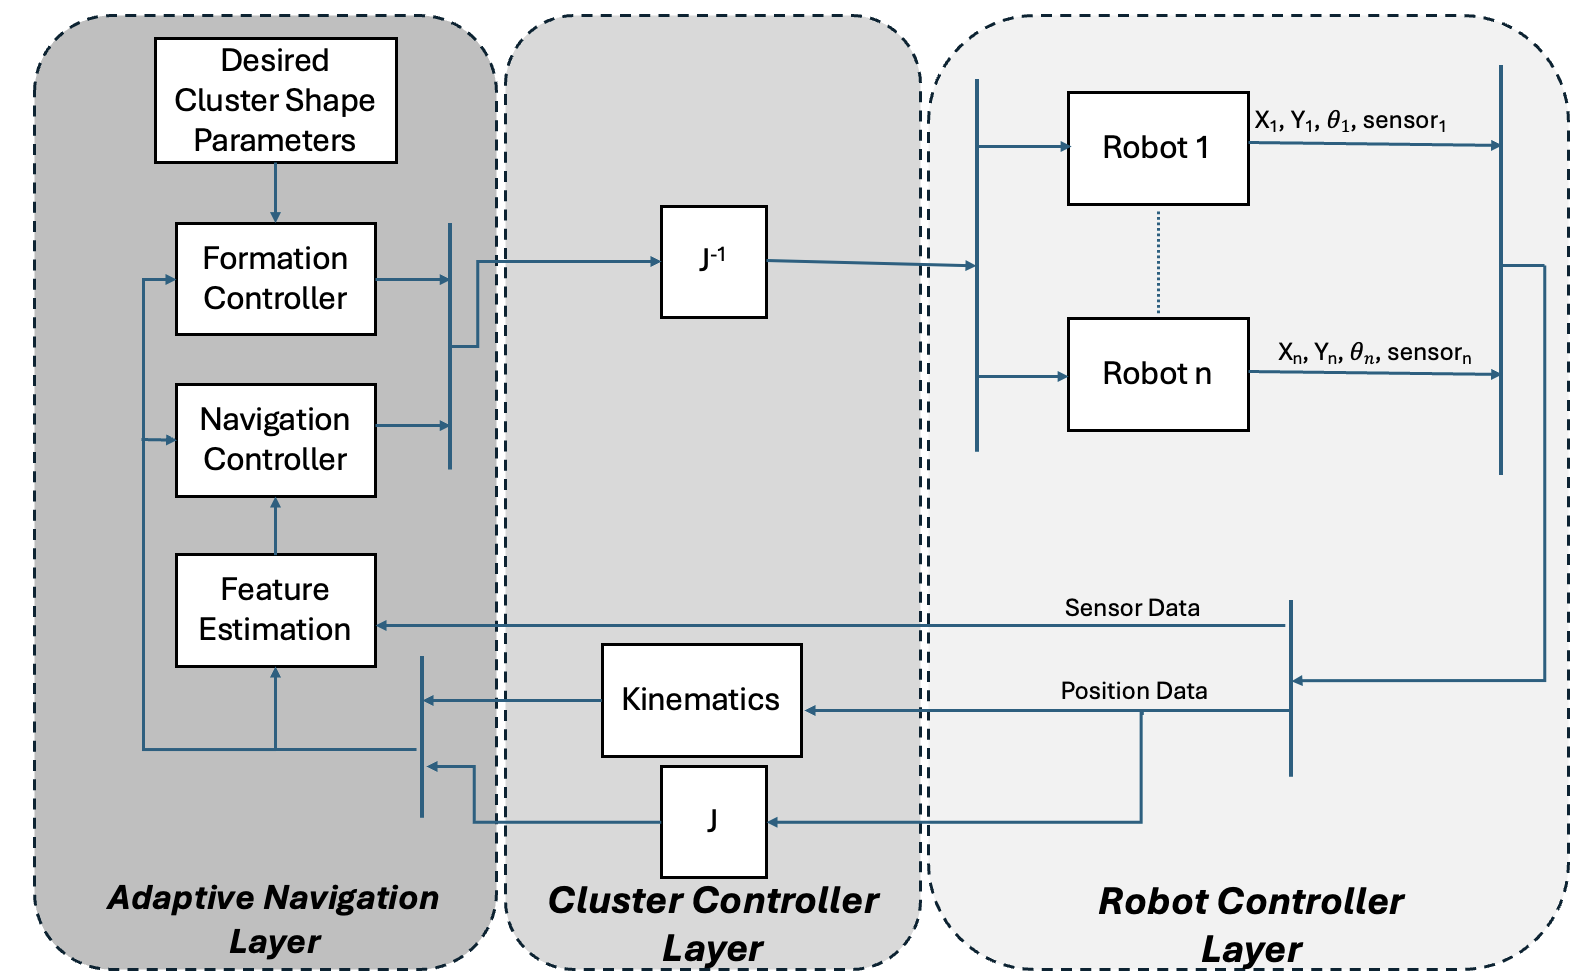
\includegraphics[width=\columnwidth]{figures/control_architecture.png}
    \caption{Three-layer control architecture. The adaptive navigation
    layer (left) estimates the field and generates the cluster command, the
    cluster controller layer (center) maps between cluster and robot space,
    and the robot controller layer (right) actuates each robot and reports
    its position and field sample.}
    \label{fig:control_architecture}
\end{figure}

\begin{figure}[!tb]
    \centering
    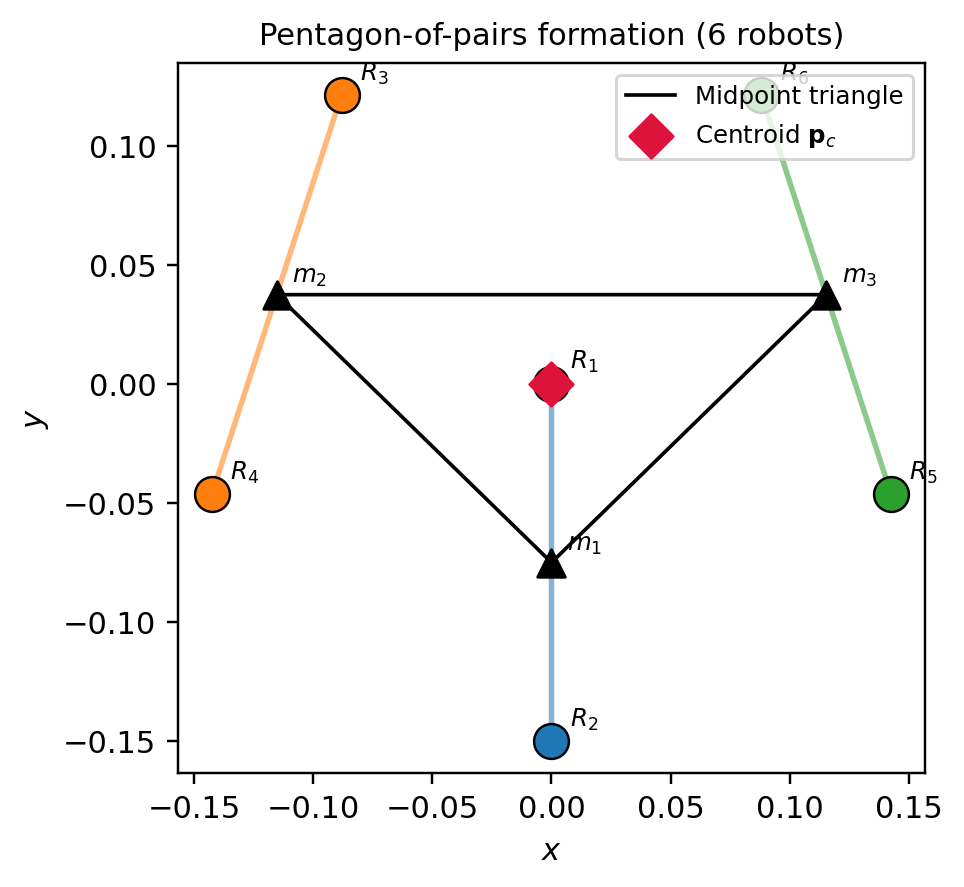
\includegraphics[width=0.85\columnwidth]{figures/pentagon_formation.png}
    \caption{Pentagon-plus-center formation. Robot 1 sits at the centroid
    $\mathbf{p}_c$ and robots 2 to 6 on a ring (dotted). The cluster
    variables shown are the pair separations $L_2$, $L_3$, $L_4$, a pair
    orientation $\theta_3$, the SAS parameters $(p, \beta, q)$ of the
    triangle of pair midpoints (squares), and the heading $\theta_c$.}
    \label{fig:pentagon}
\end{figure}

Each robot follows its velocity command through a first-order lag,
discretized at control period $\Delta t$ as the update
$\mathbf{v} \leftarrow \alpha_{\text{mom}}\mathbf{v} + (1 -
\alpha_{\text{mom}})\mathbf{v}^{\text{des}}$ with
$\alpha_{\text{mom}} = e^{-\Delta t/\tau}$. A Python simulation integrates
each robot's position by explicit Euler at the same period. This momentum model was
identified in \cite{10} on the Decabot indoor omnidirectional testbed
\cite{31,32}, and $\alpha_{\text{mom}} = 0.7$ at $\Delta t = 0.1$~s gives
$\tau \approx 0.28$~s, consistent with the identified lag. Each robot also
carries a speed limit and a stiction floor. Table~\ref{tab:params} gives
the two operating points, fixed across all experiments unless noted.

\begin{table}[!t]
\caption{Operating points. The double-gyre column is non-dimensional,
with one time unit equal to one second of the Decabot's identified
dynamics. Section~\ref{sec:ocean_sim} converts the ocean column to
physical units.}
\label{tab:params}
\centering
\begin{tabular}{llll}
\hline
Parameter & Double gyre & Ocean & Units \\
\hline
$c_{\max}$              & 0.04  & 0.033  & length/time \\
$k$                     & 3.0   & 1.94   & none \\
$\rho$                  & 0.075 & 0.098  & length (5.0 km) \\
$v_{\text{max,robot}}$  & 0.3   & 0.3    & length/time \\
$v_{\text{stiction}}$   & 0.025 & 0.002  & length/time \\
$\alpha_{\text{mom}}$   & 0.7   & 0      & none \\
$\varepsilon_{\text{raw}}$ & $10^{-3}$ & $10^{-3}$ & $1/\text{time}^2$ \\
$\varepsilon_{\dim}$    & 0.025 & 0.025  & length$^2$ \\
$g_\perp$               & 1.0   & 1.0    & length$^2$ \\
$s_{\mathrm{latch}}$     & 0.05  & 0.3    & 1/time \\
$g_{\text{capture}}$    & 0.15  & 0.15   & 1/(time$\cdot$length) \\
$r_{\text{band}}$       & 0.05  & 0.05   & 1/time \\
\hline
\end{tabular}
\end{table}

\subsection{The $D$ Tracker}
\label{sec:sep_controller}

The $D$ tracker is built for a mountain pass in $D$. Two minima are
joined by a trench that runs over a saddle point of $D$, the crest.
Around the crest the landscape is a hyperbolic paraboloid, curving up
across the trench and down along it. On the benchmark the separatrix is
such a trench, with the minima at the flow saddles
(Fig.~\ref{fig:dg_fields}(b)). The tracker drives the centroid onto the
trench and along it, over the crest, and down toward the next minimum.

A trench is taken here in the height-ridge sense \cite{33}, a curve on
which the gradient is orthogonal to a Hessian eigenvector with positive
eigenvalue. The tracker reads this frame from
$\hat{\mathbf{H}}_{D,0}\mathbf{w}_j = \lambda_j \mathbf{w}_j$, with
$\|\mathbf{w}_j\| = 1$, $\lambda_1 \leq \lambda_2$, $\mathbf{w}_2$ across
the trench, and $\mathbf{w}_1$ along it, signed by
$\hat{\mathbf{v}}_0^\top \mathbf{w}_1 \geq 0$ to point downstream. Here
$\hat{\mathbf{v}}_0 = (\hat{a}_1, \hat{b}_1)$ is the measured flow at the centroid. The
identification is exact on the benchmark, where $\mathbf{H}_D$ is
diagonal, and approximate in general.

A full Newton step $-\hat{\mathbf{H}}_{D,0}^{-1}\hat{\mathbf{g}}_0$ leads
to the stationary point of the fitted hyperbolic paraboloid, which would
stop the cluster at the crest. The tracker keeps only its across-trench
component and sets the along-trench speed separately. It uses the
along-trench gradient away from the crest, and the measured flow near
it, where that gradient vanishes. The crest is detected by a
shallow-determinant band $\mathcal{B}$, the set of points where
\begin{equation}
    |\hat{D}_0| < \varepsilon_{\mathrm{raw}}
    \quad\text{or}\quad
    \frac{|\hat{D}_0|}{\|\hat{\mathbf{H}}_{D,0}\|_F}
        < \varepsilon_{\dim},
    \label{eq:band}
\end{equation}
for an absolute threshold $\varepsilon_{\mathrm{raw}}$ on the fitted
determinant and a relative threshold $\varepsilon_{\dim}$ on its depth
against curvature. The relative
test is in units of length squared, so the band scales with the
landscape, and the absolute test catches small $|\hat{D}_0|$ where the
curvature is also small and the ratio is not. The band surrounds the
zero set of $D$, so detection assumes the crest lies within it. Since
$D = s_1 s_2 + \omega^2/4$, this holds where strain and vorticity nearly
balance at the crest. The cluster may also cross the band
during acquisition, where a trigger changes only the along-trench
speed.

The band test selects the along-trench speed,
\begin{equation}
    v_\parallel =
    \begin{cases}
        \hat{\mathbf{v}}_0^\top \mathbf{w}_1,
            & \mathbf{p}_c \in \mathcal{B}, \\[6pt]
        \dfrac{|\mathbf{w}_1^\top \hat{\mathbf{g}}_0|}{|\lambda_1|},
            & \text{otherwise},
    \end{cases}
    \label{eq:vpar}
\end{equation}
and the command, scaled by a navigation gain $k$, with each channel saturated at speed
$c_{\max}$ by $\mathrm{sat}(c) = c_{\max}\tanh(c/c_{\max})$, is
\begin{equation}
    \dot{\mathbf{p}}_c = k\Bigl[
    \underbrace{\mathrm{sat}(v_\parallel)\,\mathbf{w}_1}_{\text{along the trench}}
    + \underbrace{\mathrm{sat}\!\left(-\frac{\mathbf{w}_2^\top
      \hat{\mathbf{g}}_0}{\lambda_2}\right)\mathbf{w}_2}_{\text{across the trench}}\Bigr].
    \label{eq:d_law}
\end{equation}
The saturation caps the centroid speed at $\sqrt{2}\,k\,c_{\max}$.
Both branches of (\ref{eq:vpar}) are nonnegative, so the along-trench
motion never opposes the flow.

When $\hat{\mathbf{H}}_{D,0}$ is definite the trench frame is undefined.
The tracker then reverts to the signed Newton step
$\sum_j \mathrm{sat}(-\mathbf{w}_j^\top\hat{\mathbf{g}}_0/
\lambda_j)\mathbf{w}_j$ off the band and to the saturated flow on it.
That step settles at the fitted extremum, a minimum on a
positive-definite fit and a maximum on a negative-definite one. Since $D$
curves upward across a trench, no maximum lies on the pass, and the same
sign test is the capture condition,
\begin{equation}
    \lambda_1 \lambda_2 \geq 0,
    \label{eq:d_capture}
\end{equation}
which the true $D$ meets at each minimum of the pass.

Near the trench, with $n$ the signed distance across it, the across-trench
channel of (\ref{eq:d_law}) reduces to
$\dot{n} = \mathbf{w}_2^\top\dot{\mathbf{p}}_c = -k\,\mathrm{sat}(a_\perp n)$,
where $a_\perp = \kappa_\perp/\hat{\kappa}_\perp$ compares the true
transverse curvature with its fitted value $\hat{\kappa}_\perp = \lambda_2$.
Assuming the cluster realizes $\dot{\mathbf{p}}_c$ \cite{37,3}, the
Lyapunov function $V = \tfrac{1}{2}n^2$ gives
$\dot{V} = -k\,n\,\mathrm{sat}(a_\perp n)$, which is negative for
$n \neq 0$ whenever $\lambda_2 > 0$. The cluster therefore returns to the
trench. A disturbance on $\dot{n}$, such as a frame's transport velocity,
leaves $n$ bounded while it stays below the largest across-trench speed
$k\,c_{\max}$.

\subsection{The $s_1$ Tracker}
\label{sec:s1_controller}

The $s_1$ tracker is built for a mountain pass in $s_1$. Two
minima are joined by a trench that runs over a crest. In incompressible
flow $s_1 = -r \leq 0$, which is zero only at an isotropic point, where
the strain vanishes. Such a point is in general an isolated peak, so no
trench crosses it. The crest is instead a smooth saddle with $r > 0$, as
it is for $D$. In special flows, such as one whose shear strain vanishes
identically, the isotropic points form curves, and the crest can sit on
one at a kink of $s_1$. Where the vorticity vanishes, $D = -s_1^2$ and
the two fields share the trench.

The fitted $\hat{s}_1$ is concave for every field and formation
(Section~\ref{sec:surrogates}). Unlike $\hat{D}$, it never shows the
upward curvature a trench has across it, so no Newton step is available.
The tracker instead builds both channels from $\nabla\hat{s}_1$ and the
strain eigenframe.

On an OECS the trench tangent is a strain eigenvector, $\mathbf{e}_2$
on an attracting segment and $\mathbf{e}_1$ on a repelling one, so no
fixed choice serves both kinds of segment. On the trench the
transverse derivative of $s_1$ vanishes, so away from a stationary point
$\nabla\hat{s}_1$ lies almost along the trench. The tangent is the
eigenvector most nearly parallel to it, signed against a reference,
\begin{equation}
    \mathbf{t}_{\mathrm{raw}} =
    \arg\max_{\mathbf{e} \in \{\mathbf{e}_1, \mathbf{e}_2\}}
    \bigl\lvert \nabla\hat{s}_1^\top \mathbf{e} \bigr\rvert,
    \qquad
    \mathbf{t} = \mathrm{sgn}\bigl(\mathbf{t}_{\mathrm{ref}}^\top
    \mathbf{t}_{\mathrm{raw}}\bigr)\,\mathbf{t}_{\mathrm{raw}},
    \label{eq:tangent_select}
\end{equation}
where $\mathbf{t}_{\mathrm{ref}}$ is the previous step's tangent, or
$\hat{\mathbf{v}}_0$ on the first ride step (Fig.~\ref{fig:s1_channels}(a)). If $\hat{r}$ falls below a
strain floor $r_{\mathrm{band}}$ on that first step, the eigenframe is
unresolved and $\mathbf{t}$ is taken along $\hat{\mathbf{v}}_0$. The measured flow is not
objective, so it seeds the ride direction only once. Afterward,
estimation error can reverse the ride, whereas the $D$ tracker's
along-trench motion never opposes the flow.

The command is gradient descent, $-k\,\mathrm{sat}(g_\perp\nabla\hat{s}_1)$
with transverse gain $g_\perp$, where $\mathrm{sat}$ now saturates a
vector's magnitude and preserves its direction. Once $\hat{s}_1$ first
falls below the latch depth $-s_{\mathrm{latch}}$, the tracker rides,
\begin{equation}
    \dot{\mathbf{p}}_c = k\bigl[
    c_{\max}\tanh(1)\,\mathbf{t}
    - \mathrm{sat}\!\bigl(g_\perp\,\mathbf{P}\,\nabla\hat{s}_1\bigr)\bigr],
    \quad
    \mathbf{P} = \mathbf{I} - \mathbf{t}\mathbf{t}^\top.
    \label{eq:s1_law}
\end{equation}
The projector removes
the along-trench component of the gradient
(Fig.~\ref{fig:s1_channels}(b)), so the cluster descends only across the
trench while riding along it at speed $k\,c_{\max}\tanh 1$. The latch
depth is small relative to the well depth, so from most starts the ride
begins at the first step, and projected descent carries the cluster onto
the trench.

The tracker also stops at a minimum. The concave fit cannot certify one,
so the capture test is built on the gradient. The fitted gradient tracks
the true gradient even where the fitted curvature has the wrong sign.
Each end of the trench is a true two-dimensional minimum of $s_1$, so a
vanishing gradient suffices. Capture requires
$\|\nabla\hat{s}_1\| < g_{\mathrm{capture}}$, with
$\hat{r} > r_{\mathrm{band}}$ to exclude an isotropic point and
$\hat{s}_1 < -4s_{\mathrm{latch}}$ to exclude a shallow flat spot. The
tracker then drops the ride term and descends $\hat{s}_1$, holding the
cluster at the minimum until $\hat{s}_1$ rises back above
$-s_{\mathrm{latch}}$.

\begin{figure}[!tb]
    \centering
    \includegraphics[width=\columnwidth]{figures/s1_channels.png}
    \caption{The two channels of the $s_1$ tracker, on the benchmark
    trench at $x = 0$. (a) Tangent selection by
    (\ref{eq:tangent_select}). At each sample the strain eigenframe is
    drawn, the selected eigenvector heavy and the rejected one light,
    with $\nabla\hat{s}_1$ in orange. The argmax takes
    $\mathbf{e}_2$ on the attracting segment and $\mathbf{e}_1$ on the
    repelling segment, swapping through the isotropic point at the origin.
    (b) The command. Travel along $\mathbf{t}$ is open loop at cruise
    speed, while $\mathbf{P}$ removes the along-trench component of the
    gradient so descent acts only across the trench.}
    \label{fig:s1_channels}
\end{figure}

Near the trench, the across-trench channel of (\ref{eq:s1_law})
reduces to the $D$ tracker's $\dot{n} = -k\,\mathrm{sat}(a_\perp n)$,
with $\kappa_\perp$ now the transverse curvature of $s_1$ and
$a_\perp = g_\perp\kappa_\perp$. No fitted curvature enters, so
$a_\perp > 0$ wherever the trench curves upward across it, including at
a smooth crest. The restoring term is lost only where $\kappa_\perp$
vanishes, as where a curve of isotropic points crosses the trench. There
the ride carries the cluster across on the tangent alone.

The tangent changes eigenvector only at an isotropic point, and the rule
follows the swap with no dedicated test, since $\nabla\hat{s}_1$ stays
large on either side of the kink (Fig.~\ref{fig:s1_channels}(a)). On a
trench that is not an OECS, the rule takes the nearer eigenvector. It is
least reliable near a minimum or a smooth crest, where $\nabla\hat{s}_1$
vanishes.


\section{Double-Gyre Benchmark}
\label{sec:dg_bench}

\subsection{Setup}

The double-gyre experiments use the steady field of
Section~\ref{sec:dg_example} ($A = 0.1$) on $[-1, 1] \times
[-0.5, 0.5]$. All trials use the nominal
formation with ring radius $\rho = 0.075$; trials vary only the initial heading, drawn uniformly from $[0, 2\pi)$
in the Monte Carlo sweeps and zero in the noise-free runs. The latch
depth $s_{\mathrm{latch}} = 0.05$ is a small fraction of the well depth
$\pi^2 A \approx 0.987$.

\subsection{Clean Runs}
\label{sec:disc_clean}

\begin{figure}[!tb]
    \centering
    \includegraphics[width=0.88\columnwidth]{figures/traverse_vs_logic_c_seven.png}
    \caption{$s_1$ tracker versus $D$ tracker from seven matched starts
    ($\bullet$), noise-free, at S1 $(-0.10, 0.30)$, S2 $(0.15, 0.25)$, S3 $(0, 0.35)$,
    S4 $(0, 0)$, S5 $(0, -0.25)$, S6 $(0.15, -0.15)$, and S7 $(0.10, -0.20)$. From above the origin both
    traverse the same network through the isotropic point there. The $s_1$ tracker captures at the far saddle ($\times$), while the
    $D$ tracker continues onto the crossing wall trench past each saddle
    it reaches, ending at the squares. }
    \label{fig:traverse_vs_logic_c}
\end{figure}

\begin{figure}[!tb]
    \centering
    \includegraphics[width=0.82\columnwidth]{figures/separatrix_formation_seven.png}
    \caption{The six robots from start S1 (star) under both trackers,
    zoomed to the separatrix $x = 0$ (dashed). Thin lines are robot
    paths and the heavy line is the centroid. Outlines mark the
    pentagon-plus-center formation at the start, during the ride, and at
    the far saddle ($\times$).}
    \label{fig:formation}
\end{figure}

These runs test acquisition, traversal, and the terminal step. Clean trials
run 400 to 600 steps and stop at domain exit or, for the $D$ tracker,
150 steps after first saddle contact. A run acquires the network at the first of ten
consecutive steps with its centroid within 0.05 of the separatrix $x = 0$.

Both ran noise-free from seven matched starts
(Fig.~\ref{fig:traverse_vs_logic_c}). Three lie on the separatrix, at heights 0.35, 0, and $-0.25$. Four lie off it by $1.3\rho$ or $2\rho$, two above the origin and two below, and none of these straddles the separatrix at the first step. Both trackers acquire the network from all seven in 0 to 10 steps. Runs from above the origin then ride the same segments in the same direction and cross the isotropic point at the origin, with the formation straddling the separatrix throughout (Fig.~\ref{fig:formation}). A run
acquiring above the origin therefore rides an attracting OECS to that
point and continues onto a repelling one, on the same primitive and scalar
trench throughout. On this field neither needs a dedicated rule at the
crossing, and the $s_1$ tracker rides through the origin on ordinary
tangent selection.

The primitives part only at the terminal step. The $s_1$ tracker settles within 0.011 to 0.022 of
$\mathbf{p}^*_1 = (0, -0.5)$ in all seven runs. The
$D$ tracker passes within 0.02 of $\mathbf{p}^*_1$ and continues onto the
crossing wall trench. Over the outer half of each segment the true
$\mathbf{H}_D$ is positive definite, but
the fitted Hessian of (\ref{eq:hess_det}), which omits the third-derivative terms, stays indefinite there, and the traversal relies on that. The capture test
(\ref{eq:d_capture}) fires only near the flow saddles and domain
corners, where second derivatives vanish. There truncation error sets the
sign of the fitted eigenvalues, so the test fires only intermittently.


\subsection{Behavior Under Noise}
\label{sec:disc_noise}

\begin{figure*}[!p]
    \centering
    \includegraphics[width=\textwidth]{figures/noise_seven_starts.png}
    \caption{Far-saddle success of both trackers from the seven starts of
    Fig.~\ref{fig:traverse_vs_logic_c}, one per row, $10^4$ trials per point,
    with each tracker's straddle retention (counted on successful trials)
    dashed. S1 and S2 start off the separatrix above the origin, S3, S4, and S5
    on it, and S6 and S7 off it below the origin. Each inset marks the start
    (dot) in the basin, with the separatrix dashed and the far saddle
    $\mathbf{p}^*_1$ starred. The dotted line marks 50\% and the ticks each
    tracker's crossing. (a) Against $\sigma_{uv}$, $\sigma_p = 0$. (b) Against
    $\sigma_p$, $\sigma_{uv} = 0$.}
    \label{fig:flip_resolution}
\end{figure*}

Both primitives sweep measurement and position noise separately from the
seven starts of Fig.~\ref{fig:traverse_vs_logic_c}, at $10^4$ trials per
noise level from independent headings (Fig.~\ref{fig:flip_resolution}).
Noise-sweep trials run up to 500 steps and stop at task completion or domain
exit. Success is contact within 0.06 of the far saddle
$\mathbf{p}^*_1 = (0, -0.5)$, and each trial also records straddle retention.
A trial straddles when the robots fall on both sides of the separatrix, and
retention requires it never stop once started, the failure \cite{26}
reports. An off-separatrix start counts retention from its first straddle.
Holding one target fixed makes a settle at the near saddle a directional
failure rather than a loss of the structure. Without noise, both reach
$\mathbf{p}^*_1$ in all $10^4$ trials from every start, except the $s_1$
tracker from the origin, at 99.2\%.

Above the origin, noise favors the $D$ tracker by about four times, whether
the start lies on the separatrix or off it. The $D$ tracker crosses 50\% at
$\sigma_{uv} \approx 0.0076$ to $0.0078$ from S1 through S4, where
$\nabla\hat{D}$ stops being informative along the separatrix
($\sigma_{uv} \approx 0.0047$ to $0.0085$). The $s_1$ tracker crosses at
$\sigma_{uv} \approx 0.0019$ to $0.0021$ from S1, S2, and S3
(Fig.~\ref{fig:flip_resolution}(a)). Under position noise the ordering
holds, $\sigma_p \approx 0.0081$ to $0.0082$ against $0.0023$ to $0.0032$
(Fig.~\ref{fig:flip_resolution}(b)).

At the origin and below it the margin narrows. From the origin the $s_1$
tracker crosses at $\sigma_{uv} \approx 0.0041$. Below it, the $s_1$ tracker's
success flattens between 50 and 80\% while its retention keeps falling,
because a trial that loses the straddle on a short ride often still reaches
$\mathbf{p}^*_1$. Retention is therefore the measure there. Its 50\%
crossings give the $D$ tracker 1.5 to 2.6 times the $s_1$ tracker's
tolerance below the origin, 3.1 at it, and 4.4 to 4.7 above it. The $D$
tracker itself tolerates more noise on the short ride from S5,
$\sigma_{uv} \approx 0.0114$, and less from S6 and S7, $\sigma_{uv} \approx
0.0043$ and $0.0047$.

The $D$ tracker loses tolerance below the origin only where it must acquire
the separatrix there. By (\ref{eq:det_analytic_main}), $\mathbf{H}_D$ is
indefinite only for $|y| < 0.25$, and over the outer half of each segment
only truncation keeps the fitted Hessian indefinite
(Section~\ref{sec:disc_clean}). S6 and S7 drift downstream while acquiring
and reach the separatrix near $y = -0.30$, inside that outer half. At
$\sigma_{uv} = 0.005$ the fit turns definite before acquisition in 83\% and
75\% of their trials, and the tracker reverts to the signed Newton step
(Section~\ref{sec:sep_controller}). Those trials reach $\mathbf{p}^*_1$ in
27\% and 36\% of cases, against 68\% for the rest. S1 and S2 revert in 68\%
and 51\% of trials but reach the separatrix near $y = 0.24$ and $0.14$,
inside the indefinite band, and succeed as often either way. No noise-free
trial reverts.

We attribute the $s_1$ tracker's fragility to how long a sign decision
persists before a new measurement checks it, rather than to per-cycle
estimation accuracy. The $D$ tracker re-signs $\mathbf{w}_1$ against
$\hat{\mathbf{v}}_0$ every cycle, while the $s_1$ tracker carries the sign in
state through $\mathbf{t}_{\mathrm{ref}}$. Objectivity rules out the fitted
curvature (Section~\ref{sec:surrogates}), the measured flow
(Section~\ref{sec:rotating}), and a world axis as sign references, and
traversal rules out the along-trench component of $\nabla\hat{s}_1$, which
reverses at the along-trench maximum the ride must cross, so we use the
primitive's own prior output.

Where the sign is lost depends on height. On the trench, tangent selection
rests on the along-trench slope $|\partial s_1/\partial y| = \pi^3 A|\cos\pi
y|$ from (\ref{eq:s1_analytic_main}), which vanishes at both saddles. One
step that selects the transverse eigenvector leaves $\mathbf{t}_{\mathrm{ref}}$
across the trench, and the next step's sign is then arbitrary. At
$\sigma_{uv} = 0.002$ the rate of first reversals per riding step is 0.002 to
0.004 for $|y| < 0.2$ and rises to 0.06 to 0.20 within 0.1 of either saddle.
A reversal carries the cluster back toward $\mathbf{p}^*_2$, and 91 to 94\% of
failures end within 0.06 of it. A start near $\mathbf{p}^*_2$ therefore begins
in the high-rate band. Success at this level falls with start height, from
0.70 to 0.78 at and below the origin to 0.54, 0.51, and 0.44 from S2, S1, and
S3.

From S3, straddle retention stays within five points of success for the $D$
tracker but falls further below it for the $s_1$ tracker, 47.6\% against
71.5\% at $\sigma_{uv} = 0.0015$. Most $s_1$ trials from S3 that lose the
straddle do so within 0.1 of the origin, where the $s_1$ trench loses its
transverse curvature (Section~\ref{sec:s1_controller}).

\subsection{Behavior Under a Rotating Observer}
\label{sec:rotating}

\begin{figure}[!tb]
    \centering
    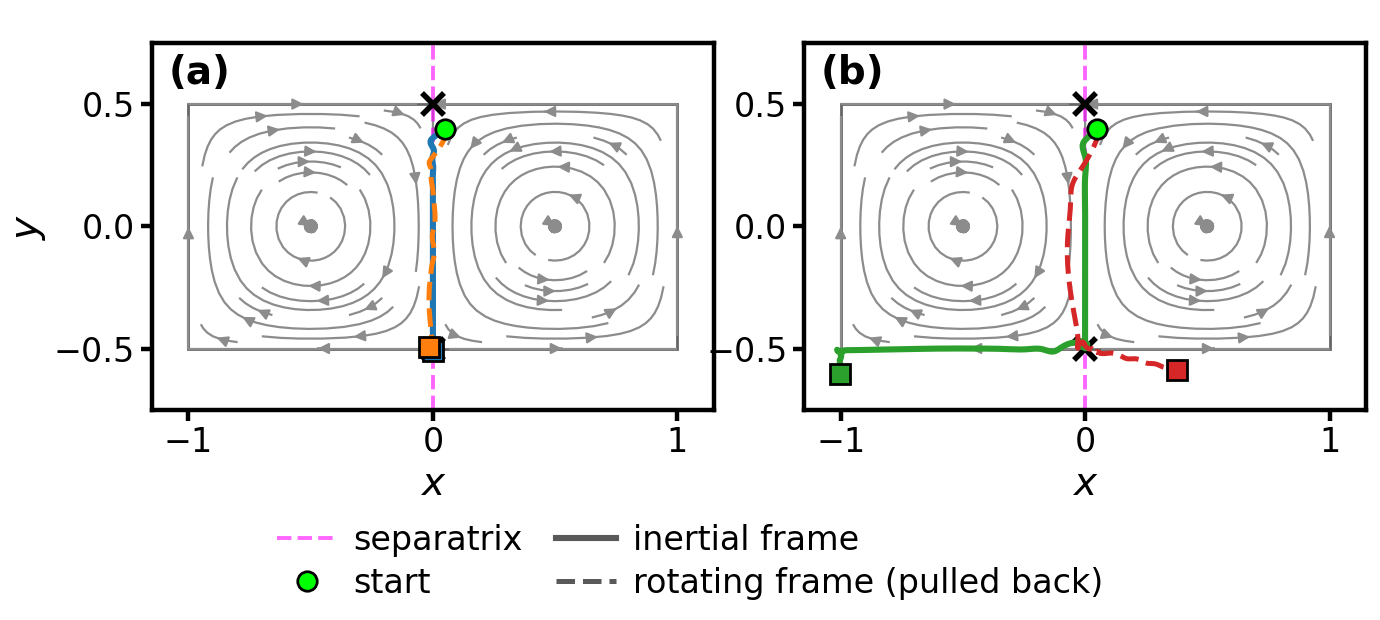
\includegraphics[width=\columnwidth]{figures/objectivity_traverser.png}
    \caption{Objectivity trial, both primitives started from
    $(0.05, 0.40)$ and run in the inertial frame (solid) and in a
    frame rotating at $\Omega = 0.23$ (dashed, pulled back to
    inertial coordinates). (a) The $s_1$ tracker's two runs coincide
    and capture at the same saddle. (b) The $D$ tracker's rotating-frame
    run loses the straddle across the crest (inset), the artifact
    predicted by (\ref{eq:D_not_objective}), and rejoins near the far
    saddle.}
    \label{fig:oecs_objectivity}
\end{figure}

A cluster can sense the water without error and still see the flow from a
rotating frame. This happens when each robot senses water velocity relative
to itself and adds its own velocity, differenced from position fixes
expressed in drifting axes. The flow the cluster measures is then
\[
\mathbf{v}'(\mathbf{p}', t) =
\mathbf{Q}\mathbf{v}(\mathbf{Q}^\top \mathbf{p}') + \Omega\,(-y', x')^\top ,
\]
the physical flow seen in rotated axes plus the transport velocity of a
frame rotating clockwise at rate $\Omega$. A cluster whose sensors instead
report $\mathbf{Q}\mathbf{v}$ while its relative positions stay in true
axes fits $\mathbf{Q}\mathbf{J}$, which leaves the $D$ field unchanged but
tilts the strain eigenframe.

Both primitives were run from $(0.05, 0.40)$, just inside the upper saddle,
on the same physical double gyre, once in the inertial frame and once in a
frame rotating at $\Omega = 0.23$. The rate is about 23\% of the flow's
peak strain rate, $\Omega/(\pi^2 A) \approx 0.23$. It keeps the structure's
apparent speed along the tracked path, $\Omega\lVert\mathbf{p}\rVert \leq
0.11$, inside the command authority $k\,c_{\max} = 0.12$. That is the
condition under which the offset from the trench stays bounded
(Section~\ref{sec:sep_controller}), so the cluster is fast enough to follow the structure in either
frame. Rotating-frame trajectories are pulled back to inertial coordinates
and compared with the same primitive's inertial run.

In the rotating frame the $s_1$ tracker's run nearly coincides with its
inertial run (Fig.~\ref{fig:oecs_objectivity}(a)). Between acquisition and
the far saddle it stays within 0.016 of the separatrix, against 0.010 in
the inertial frame. It keeps the straddle throughout, and both runs capture
at the same saddle, $\mathbf{p}_1^*$.

The $D$ tracker's rotating-frame run departs from its inertial run
(Fig.~\ref{fig:oecs_objectivity}(b)). It is displaced from the separatrix
by up to 0.084, against 0.010 in the inertial frame. Across the crest it
loses the straddle for 36 steps, with all six robots on one side of the
separatrix, the failure \cite{26} reports. It rejoins the separatrix near
$\mathbf{p}_1^*$. In a sweep over the rate, the $D$ tracker first loses the
straddle at $\Omega \approx 0.21$. There $\Omega\lVert\mathbf{p}\rVert$ at
the crest is a sixth of the command authority, so the cluster has speed to
spare when the straddle breaks.

The trackers diverge because the frame's spin enters the $D$ field, while
the strain only co-rotates. The rotating frame adds a uniform vorticity $2\Omega$, which
shifts the $D'$ landscape by (\ref{eq:D_not_objective}). It also adds its
transport velocity to the measured flow, so both terms of the $D$ tracker
steer on a frame artifact. On the separatrix the added term
$\Omega\omega$ is zero, but its transverse gradient
$\partial_x\omega = 2\pi^3 A\sin\pi y_f$ is not, so $\Omega\omega$ tilts
$D'$ across the trench. Against the trench's transverse curvature
$2\pi^6 A^2$, the tilt moves the trench by
$\Omega\sin(\pi y_f)/(\pi^3 A)$. The displacement is largest at the origin
and zero at the saddles, which is why the $D$ tracker's run rejoins the
separatrix near $\mathbf{p}_1^*$.

The $s_1$ tracker's tests are scalar inequalities in quantities a rotation
leaves invariant, so its command co-rotates with the frame. Its residual is
the frame's transport velocity, bounded under the authority condition above. Its one non-objective input is the tangent
seed, read from the measured flow on the first ride step. The seed fixes
the ride direction, and the two frames agree on it while
$\Omega\lVert\mathbf{p}_{\text{seed}}\rVert <
\lvert\hat{\mathbf{v}}_0^\top\mathbf{t}_{\text{raw}}\rvert$, that is, while
the transport velocity at the seed point is smaller than the measured
flow's component along $\mathbf{t}_{\text{raw}}$.

\section{Santa Barbara Channel Trial}
\label{sec:ocean}

\subsection{Setup}
\label{sec:ocean_sim}

The ocean experiment uses hourly surface-current frames for the Santa
Barbara Channel from the HFRNet U.S.~West~Coast Radial-to-Total Vector
product \cite{34,38}, on the $2$~km grid, which is public. The record is the one \cite{26} uses, the same network over the same 28-h window, 29 frames from May 16, 2012 08:00 GMT to May 17, 2012 12:00 GMT. Kularatne and Hsieh track a time-reversed attracting boundary in the same channel's May 2012 currents \cite{29}.
Frames are interpolated linearly in time and bilinearly in space. World
coordinates on $[-0.65, 0.65]^2$ map affinely onto a region centered on
$(34.2^{\circ}\mathrm{N}, 120.4^{\circ}\mathrm{W})$. Radar coverage is partial, and 74 to 87\%
of the water cells in that region are valid in each frame. Missing cells,
including land inside the coverage, are filled by linear interpolation
across the valid ones, and the field is zero beyond the valid data. A run
ends at landfall, the first step at which any robot lies over land on the
Natural Earth 1:10 million coastline.

Physical numbers follow from one unit block, length $L_w = 51.4$~km on
both axes and time $6000$~s, with a control period $\Delta t = 0.1$
time units, so one step advances the field by $600$~s and the
$168$-step trial covers the record. The commanded-speed cap
$\sqrt{2}\,k\,c_{\max}$ is then $0.78$~m/s, within reach of a small
autonomous surface vessel but above a buoyancy glider. With longitude
scaled by $\cos(34.2^{\circ})$ the map is a uniform dilation, so the zero
sets, trenches, and eigenframe are the physical ones. The FTLE reference
uses the same constants, over a 24-h field for Fig.~\ref{fig:ocean_ftle}
and 12~h for a persistence check. It advects a seed grid four times finer
than the data grid through the same field by fourth-order Runge-Kutta at
600~s steps, with land held at zero velocity. The seed grid covers $33.8$
to $34.7^{\circ}$N and $119.7$ to $120.7^{\circ}$W. Ridge points are the
FTLE grid points over water at or above the 95th percentile of the field.

The pentagon is enlarged to $\rho = 0.098$, $1.3\times$ the nominal radius
and $5.0$~km at this site, so the footprint spans about five cells of the
$2$~km grid rather than under four, and starts at heading $335^\circ$. At
one control cycle per ten minutes any vessel time constant is negligible,
so $\alpha_{\text{mom}} = 0$. The gain and radius set when the cluster
reaches the bifurcation of the evolving ridge, and so which branch it
meets. The latch depth $s_{\mathrm{latch}} = 0.3$ is set from this field's
$s_1$ scale. No
noise level is estimated, since the exactly determined fit leaves no
residual (Section~\ref{sec:minimality}), so the noise model is validated on the double gyre only.

\subsection{Results}
\label{sec:disc_ocean}

\begin{figure*}[!tb]
    \centering
    \includegraphics[width=\textwidth]{figures/ocean_progression_2km.png}
    \caption{$D$ and $s_1$ tracker paths from a single shared start at
    (a) 7, (b) 14, (c) 21, and (d) 28~h, each drawn up to that time, with
    dots marking the current positions. The background is the 24-h forward
    FTLE field computed offline from the same 2~km data and anchored at the
    record start. Both follow the dominant ridge from the channel entrance
    to the bifurcation, where the $D$ tracker turns onto the southeastern
    branch toward the middle island. The $D$ run stops at 24~h, when its
    first robot reaches the island.}
    \label{fig:ocean_ftle}
\end{figure*}

The field is divergent and not vorticity-free, so $s_2 = -s_1$ does not
hold and the two surrogates need not share trenches. Both were run with no
changes to the primitives, at the ocean operating point of
Table~\ref{tab:params}, from a shared start north of the channel entrance,
$(34.38^{\circ}\mathrm{N}, 120.41^{\circ}\mathrm{W})$. Over the 28-h trial
both descend through the channel entrance and track the same ridge to the
bifurcation. There the $D$ tracker turns onto the southeastern branch, and
its run stops after 24~h, when its first robot reaches the coast of the
middle island. Neither primitive has a rule for choosing a branch, so which
one the $D$ tracker takes follows from when it arrives. The $s_1$ tracker
is still descending when the record ends.

Fig.~\ref{fig:ocean_ftle} places both trials against the 24-h forward-time
FTLE field, computed offline in the style of \cite{17}. Both follow the
dominant ridge from the channel entrance to the bifurcation closely. Mean
distance from the centroid path to the nearest ridge point
is 1.5~km for the $D$ tracker and 2.1~km for the $s_1$ tracker. Past the
bifurcation the $D$ tracker continues to follow the FTLE ridge. The grid is
2~km and the formation radius 5.0~km. That ridge was available to neither,
and FTLE recomputed at four anchor times shows it persisting while the
finer structure downstream evolves.

\section{Limitations and Future Work}
\label{sec:disc_limits}

Cluster space control is centralized, requires global state, becomes intractable
for suitably large clusters, and is impractical without reliable
high-bandwidth communication among the robots \cite{30}. Distributed
consensus protocols share state only among neighbors, and event-triggered
ones only when a trigger condition fires \cite{35}, but the estimator as
built gathers all six readings on one processor each step. The claims here
are for small clusters in a limited workspace with ample bandwidth, the
regime the six-robot estimator occupies.

Two limitations sit in the estimator and its band logic. The fit is
ill-conditioned whenever the six sampling points drift toward a common
conic, and no field tested here drives the formation toward one, so the
estimator is untested in the regime its own conditioning limit
describes; the mitigation, monitoring $\kappa(\boldsymbol{\Phi})$ with a
shape-maintenance term, is not implemented. The band test carries no
hysteresis, so noise can chatter the $D$ tracker across its boundary,
which costs speed alone, since both branches share the same transverse
dynamics.

The eigenvector comparison of
Section~\ref{sec:s1_controller} weakens near the saddles. The residual risk
of a wrong branch under heavy noise is damped but not excluded by the
capture latch.

The $s_1$ tracker's passage through the origin rests on a symmetry of the benchmark and is untested without it. Its shear strain vanishes identically (Section~\ref{sec:dg_example}), so a strain eigenvector lies along the trench at every point and the trench rises to an isotropic point. Without the symmetry the eigenvector can tilt away from the trench, and the open-loop travel along $\mathbf{t}$ then pushes the cluster across it (Section~\ref{sec:s1_controller}). The crest also becomes a smooth saddle, where the tangent selection rests on a weak signal (Section~\ref{sec:s1_controller}).

The $D$ tracker assumes the crest lies in the band, where strain and vorticity nearly
balance (Section~\ref{sec:sep_controller}), since off the band the
along-trench drive vanishes at the crest. That assumption is untested off the benchmark. A rotating observer shifts the
crest by $\Omega\omega + \Omega^2$ (\ref{eq:D_not_objective}), which can
carry it out of the band. Its
capture at a minimum is also intermittent. Near a flow saddle truncation
error sets the sign of the fitted eigenvalues, and on the benchmark the
cluster passes the saddle and continues onto the wall trench
(Section~\ref{sec:disc_clean}). Acquisition where the true $\mathbf{H}_D$ is definite rests on the same
truncation, and under measurement noise it fails there more often (Section~\ref{sec:disc_noise}).

No controlled head-to-head against the straddle family \cite{26,27,28} or the onboard-FTLE strategy of \cite{29} was run. Running those methods from an off-structure start is outside their stated problems, and their robots are advected while this paper's are not, so one simulator cannot host both.
All results are simulated, and the ocean run samples the gridded product without added noise. The ocean agreement is a finding on one time-varying record, where
neither primitive has an analytic guarantee, not a guarantee for arbitrary
flows. Neither instantaneous field is guaranteed to mark the material
transport structure \cite{18}. The no-advection premise is exact for the
planned Decabot follow-on, where the field is encoded and read rather
than physically experienced \cite{32}, but on the ocean field it is an
extrapolation, untested against real advection.

Ongoing and future work targets a) extending the stability argument to
time-varying fields; b) online formation reshaping, to protect the
conditioning of $\boldsymbol{\Phi}$; c) a cubic fit from ten robots off any common cubic curve, which
recovers the third derivatives on which the true $\mathbf{H}_D$ and the
transverse curvature of an $s_1$ trench depend; d) testing both primitives on the Decabot testbed, then on surface vessels; and e) detecting a faulty robot. The exactly determined six-robot fit absorbs a bad reading without residual, but a seventh robot leaves one that a threshold test could flag, as in residual-based fault detection for multiagent consensus \cite{36}.

\section{Conclusion}

This paper has shown that a second-order fit of the local flow, from six
robots sampling at once, can be used to acquire and ride the instantaneous
coherent structures of a planar flow. The fit gives the velocity gradient
as a field over the formation, and the two adaptive navigation primitives
built on it use only synchronous local velocity measurements, with no
map, no forecast, and no assumption about the structure's identity.

The experiments give an operational selection rule. With a noisy sensor
the $D$ tracker withstands more noise than the $s_1$ tracker from every start tested, more than four times as much upstream of the isotropic point and about twice as much downstream of it. Under a rotating observer the
ranking reverses. Above a rotation rate of about a fifth of the flow's peak strain rate the $D$ tracker's formation
no longer straddles the structure, while the $s_1$ tracker keeps the
straddle and returns the same material curve in both frames. On Santa Barbara Channel currents both followed the same transport corridor
to its bifurcation, with full-run mean distances of 1.5 and 2.1~km from an FTLE ridge. A cluster with an absolute heading reference, such as a compass, GNSS
heading, or overhead tracking, should carry the $D$ tracker, which
tolerates a noisier sensor. One whose flow estimate carries its own rotation, as when robot
velocities are differenced from position fixes in drifting axes, should
carry the $s_1$ tracker, which is objective past its one seed step.

\begin{thebibliography}{99}
\itemsep 0pt plus 0.2pt
\parskip 0pt
\bibitem{1} J. Cortés and M. Egerstedt, ``Coordinated control of multi-robot
systems: A survey,'' \textit{SICE J. Control Meas. Syst. Integr.},
vol. 10, no. 6, pp. 495--503, 2017.

\bibitem{2} T. Adamek, C. A. Kitts, and I. Mas, ``Gradient-based cluster space
navigation for autonomous surface vessels,'' \textit{IEEE/ASME Trans.
Mechatronics}, vol. 20, no. 2, pp. 506--518, 2015.

\bibitem{3} C. A. Kitts, R. T. McDonald, and M. A. Neumann, ``Adaptive
navigation control primitives for multirobot clusters: Extrema finding,
contour following, ridge/trench following, and saddle point station keeping,''
\textit{IEEE Access}, vol. 6, pp. 17625--17642, 2018.

\bibitem{4} R. T. McDonald et al., ``Navigation of
scalar fronts with multirobot clusters in simulation and experiment,''
\textit{IEEE Syst. J.}, vol. 14, no. 3, pp. 3755--3766, 2020.

\bibitem{5} L. Briñón-Arranz, A. Renzaglia, and L. Schenato, ``Multirobot
symmetric formations for gradient and Hessian estimation with application to
source seeking,'' \textit{IEEE Trans. Robot.}, vol. 35, no. 3,
pp. 782--789, 2019.

\bibitem{6} P. Ögren, E. Fiorelli, and N. E. Leonard, ``Cooperative control
of mobile sensor networks: Adaptive gradient climbing in a distributed
environment,'' \textit{IEEE Trans. Autom. Control}, vol. 49, no. 8,
pp. 1292--1302, 2004.

\bibitem{7} R. T. McDonald, C. A. Kitts, and M. A. Neumann, ``Experimental
implementation and verification of scalar field ridge, trench, and saddle
point maneuvers using multirobot adaptive navigation,'' \textit{IEEE Access},
vol. 7, pp. 62950--62961, 2019.

\bibitem{8} A. Okubo, ``Horizontal dispersion of floatable particles in the
vicinity of velocity singularities such as convergences,'' \textit{Deep-Sea
Res.}, vol. 17, no. 3, pp. 445--454, 1970.

\bibitem{9} P. Keramea, K. Spanoudaki, G. Zodiatis, G. Gikas, and
G. Sylaios, ``Oil spill modeling: A critical review on current trends,
downscaling, and applications,'' \textit{J. Mar. Sci. Eng.}, vol. 9,
no. 2, art. 181, 2021.

\bibitem{10} C. Waight and C. A. Kitts, ``Adaptive navigation of multirobot
systems to critical points in 2D vector fields,'' submitted for publication.

\bibitem{11} T. Peacock and G. Haller, ``Lagrangian coherent structures: The
hidden skeleton of fluid flows,'' \textit{Phys. Today}, vol. 66, no. 2,
pp. 41--47, 2013.

\bibitem{12} M. Serra et al., ``Search and rescue at sea aided by hidden flow
structures,'' \textit{Nat. Commun.}, vol. 11, no. 1, p. 2525, 2020.

\bibitem{13} J. Das et al., ``Coordinated sampling of dynamic oceanographic
features with underwater vehicles and drifters,'' \textit{Int. J. Robot.
Res.}, vol. 31, no. 5, pp. 626--646, 2012.

\bibitem{14} S. McCammon et al., ``Ocean front detection and tracking using a
team of heterogeneous marine vehicles,'' \textit{J. Field Robot.}, vol. 38,
no. 6, pp. 854--881, 2021.

\bibitem{15} S. R. Ramp et al., ``Preparing to predict: the second autonomous
ocean sampling network (AOSN-II) experiment in the Monterey Bay,''
\textit{Deep-Sea Res. II}, vol. 56, no. 3-5, pp. 68--86, 2009.

\bibitem{16} G. Haller and G. Yuan, ``Lagrangian coherent structures and mixing
in two-dimensional turbulence,'' \textit{Physica D}, vol. 147, no. 3-4,
pp. 352--370, 2000.

\bibitem{17} S. C. Shadden, F. Lekien, and J. E. Marsden, ``Definition and
properties of Lagrangian coherent structures from finite-time Lyapunov
exponents in two-dimensional aperiodic flows,'' \textit{Physica D}, vol. 212,
no. 3-4, pp. 271--304, 2005.

\bibitem{18} G. Haller, ``Lagrangian coherent structures,'' \textit{Annu. Rev.
Fluid Mech.}, vol. 47, pp. 137--162, 2015.

\bibitem{19} M. Serra and G. Haller, ``Objective Eulerian coherent
structures,'' \textit{Chaos}, vol. 26, no. 5, p. 053110, 2016.

\bibitem{20} P. J. Nolan, M. Serra, and S. D. Ross, ``Finite-time Lyapunov
exponents in the instantaneous limit and material transport,''
\textit{Nonlinear Dyn.}, vol. 100, no. 4, pp. 3825--3852, 2020.

\bibitem{21} T. D. Harms, S. L. Brunton, and B. J. McKeon, ``Lagrangian
gradient regression for the detection of coherent structures from sparse
trajectory data,'' \textit{R. Soc. Open Sci.}, vol. 11, no. 9,
p. 240586, 2024.

\bibitem{22} J. Weiss, ``The dynamics of enstrophy transfer in two-dimensional
hydrodynamics,'' \textit{Physica D}, vol. 48, no. 2-3, pp. 273--294, 1991.

\bibitem{23} J. C. R. Hunt, A. A. Wray, and P. Moin, ``Eddies, streams, and
convergence zones in turbulent flows,'' in \textit{Proc. Summer Program,
Center Turbul. Res.}, Rep. CTR-S88, pp. 193--208, 1988.

\bibitem{24} B.-L. Hua and P. Klein, ``An exact criterion for the stirring
properties of nearly two-dimensional turbulence,'' \textit{Physica D}, vol. 113,
no. 1, pp. 98--110, 1998.

\bibitem{25} C. Dong et al., ``Oceanic mesoscale eddies,''
\textit{Ocean-Land-Atmos. Res.}, vol. 4, p. 0081, 2025.

\bibitem{26} M. Michini, M. A. Hsieh, E. Forgoston, and I. B. Schwartz,
``Robotic tracking of coherent structures in flows,'' \textit{IEEE Trans.
Robot.}, vol. 30, no. 3, pp. 593--603, 2014.

\bibitem{27} M. Michini, H. Rastgoftar, M. A. Hsieh, and S. Jayasuriya,
``Distributed formation control for collaborative tracking of manifolds in
flows,'' in \textit{Proc. Amer. Control Conf.}, pp. 3874--3880, 2014.

\bibitem{28} M. Michini, M. A. Hsieh, E. Forgoston, and I. B. Schwartz,
``Experimental validation of robotic manifold tracking in gyre-like flows,''
in \textit{Proc. IEEE/RSJ Int. Conf. Intell. Robots Syst.},
pp. 2306--2311, 2014.

\bibitem{29} D. Kularatne and M. A. Hsieh, ``Tracking attracting manifolds in
flows,'' \textit{Auton. Robots}, vol. 41, no. 8, pp. 1575--1588, 2017.

\bibitem{30} C. A. Kitts and I. Mas, ``Cluster space specification and control
of mobile multirobot systems,'' \textit{IEEE/ASME Trans. Mechatronics},
vol. 14, no. 2, pp. 207--218, 2009.

\bibitem{31} S. Tomer et al., ``A low-cost indoor testbed for multirobot
adaptive navigation research,'' in \textit{Proc. IEEE Aerosp. Conf.},
pp. 1--12, 2018.

\bibitem{32} C. Waight and C. A. Kitts, ``A functional indoor testbed for
multirobot adaptive navigation in vector field environments,'' in
\textit{Proc. ASME Int. Des. Eng. Tech. Conf.}, vol. 89251, 2025.

\bibitem{33} D. Eberly et al., ``Ridges for image analysis,''
\textit{J. Math. Imaging Vis.}, vol. 4, no. 4, pp. 353--373, 1994.

\bibitem{34} Coastal Observing Research and Development Center, Scripps
Inst. Oceanogr., ``Near-real time surface ocean velocity, U.S. West Coast,
2 km resolution,'' HFRNet, NOAA NCEI Accession
gov.noaa.nodc:IOOS-HFRadarRTVector, 2012. [Online]. Available:
\url{https://www.ncei.noaa.gov/thredds-ocean/fileServer/ioos/hfradar/rtv/2012/201205/USWC/}.
Accessed: Jul. 1, 2026.

\bibitem{35} S. Zhang, J. Liu, W. Wang, and Z. Zhang, ``Bipartite
leader-following consensus of nonlinear switched multiagent systems under
model-depended dynamic event-triggered control,'' \textit{IEEE Syst. J.},
vol. 18, no. 2, pp. 1044--1055, 2024.

\bibitem{36} R. Yang, X. Su, Y. Li, S. Zhang, and D. Zhou, ``Distributed
event-triggered simultaneous fault detection and consensus control for
multiple Lur'e systems,'' \textit{IEEE Syst. J.}, vol. 18, no. 1,
pp. 108--119, 2024.

\bibitem{37} I. Mas and C. A. Kitts, ``Obstacle avoidance policies for cluster
space control of nonholonomic multirobot systems,'' \textit{IEEE/ASME Trans.
Mechatronics}, vol. 17, no. 6, pp. 1068--1079, 2012.

\bibitem{38} E. Terrill et al., ``Data management and real-time distribution
in the HF-Radar National Network,'' in \textit{Proc. MTS/IEEE OCEANS},
Boston, MA, USA, Sep. 2006.

\end{thebibliography}

\end{document}

